\documentclass{beamer}
\mode<presentation>
\usetheme{Ilmenau}
\usepackage{graphics}
\usepackage{mathtools}
\beamertemplatenavigationsymbolsempty
\title[Advanced Numerical Methods for Neutron Star Interfaces] % (optional, only for long titles)
{Advanced Numerical Methods for \\
Neutron Star Interfaces}
\subtitle{}
\author[John Muddle - @john$\_$muddle] % (optional, for multiple authors)
{John Muddle}
\institute[University of Southampton] % (optional)
{
  Mathematical Sciences\\
  University of Southampton\\[1\baselineskip]
  Supervisor - Dr Ian Hawke

}
\date[Britgrav 2016] % (optional)
{BritGrav, 2016}
\AtBeginSection[]
{
  \begin{frame}<beamer>
    \frametitle{Outline}
    \tableofcontents[currentsection]
  \end{frame}
}
%change color fot the institute
\setbeamercolor{institute in head/foot}{fg=white}
\makeatletter
%change the footline template to include frame numbers
\defbeamertemplate*{footline}{myminiframes theme}
  {%
    \begin{beamercolorbox}[colsep=1.5pt]{upper separation line foot}
    \end{beamercolorbox}
    \begin{beamercolorbox}[ht=2.5ex,dp=1.125ex,%
      leftskip=.3cm,rightskip=.3cm plus1fil]{author in head/foot}%
      \leavevmode{\usebeamerfont{author in head/foot}\insertshortauthor}%
      \hfill%
      {\usebeamerfont{institute in head/foot}\usebeamercolor[fg]{institute in head/foot}\insertshortinstitute}%
    \end{beamercolorbox}%
    \begin{beamercolorbox}[ht=2.5ex,dp=1.125ex,%
      leftskip=.3cm,rightskip=.3cm plus1fil]{title in head/foot}%
      {\usebeamerfont{title in head/foot}\insertshorttitle\hfill \insertframenumber/\inserttotalframenumber}%<-here
    \end{beamercolorbox}%
    \begin{beamercolorbox}[colsep=1.5pt]{lower separation line foot}
    \end{beamercolorbox}
  }
\makeatother

%change look of sections in ToC
\defbeamertemplate*{section in toc}{mysections in toc}
{\leavevmode ---\,\inserttocsection\par}
\begin{document}

\begin{frame}
  \titlepage
\end{frame}
\begin{frame}
\frametitle{Acknowledgements}
I would like to thank the following:
\begin{itemize}
\item{Ian Hawke, Stephanie Erickson and Carsten Gundlach}
\item{Southampton General Relativity Group}
\item{STFC}
\item{IOP Gravity Group}
\item{Classical and Quantum Gravity}
\end{itemize}
\end{frame}
 \begin{frame}
   \frametitle{Outline}
   \tableofcontents
 \end{frame}
\section{Motivation: Neutron Stars}

\begin{frame}
\frametitle{Motivation: Binary Mergers}
\begin{columns}
\column{0.55\textwidth}
\begin{itemize}
\item{Neutron star binary mergers are strong candidates for the emission of detectable gravitational waves.}
\item{Accurate gravitational wave templates are required to directly detect gravitational waves.}
\item{Full non-linear numerical simulations are required for the plunge and merger phases.}
\item{Therefore, accurate numerical simulations are needed.}
\end{itemize}
\column{0.45\textwidth}
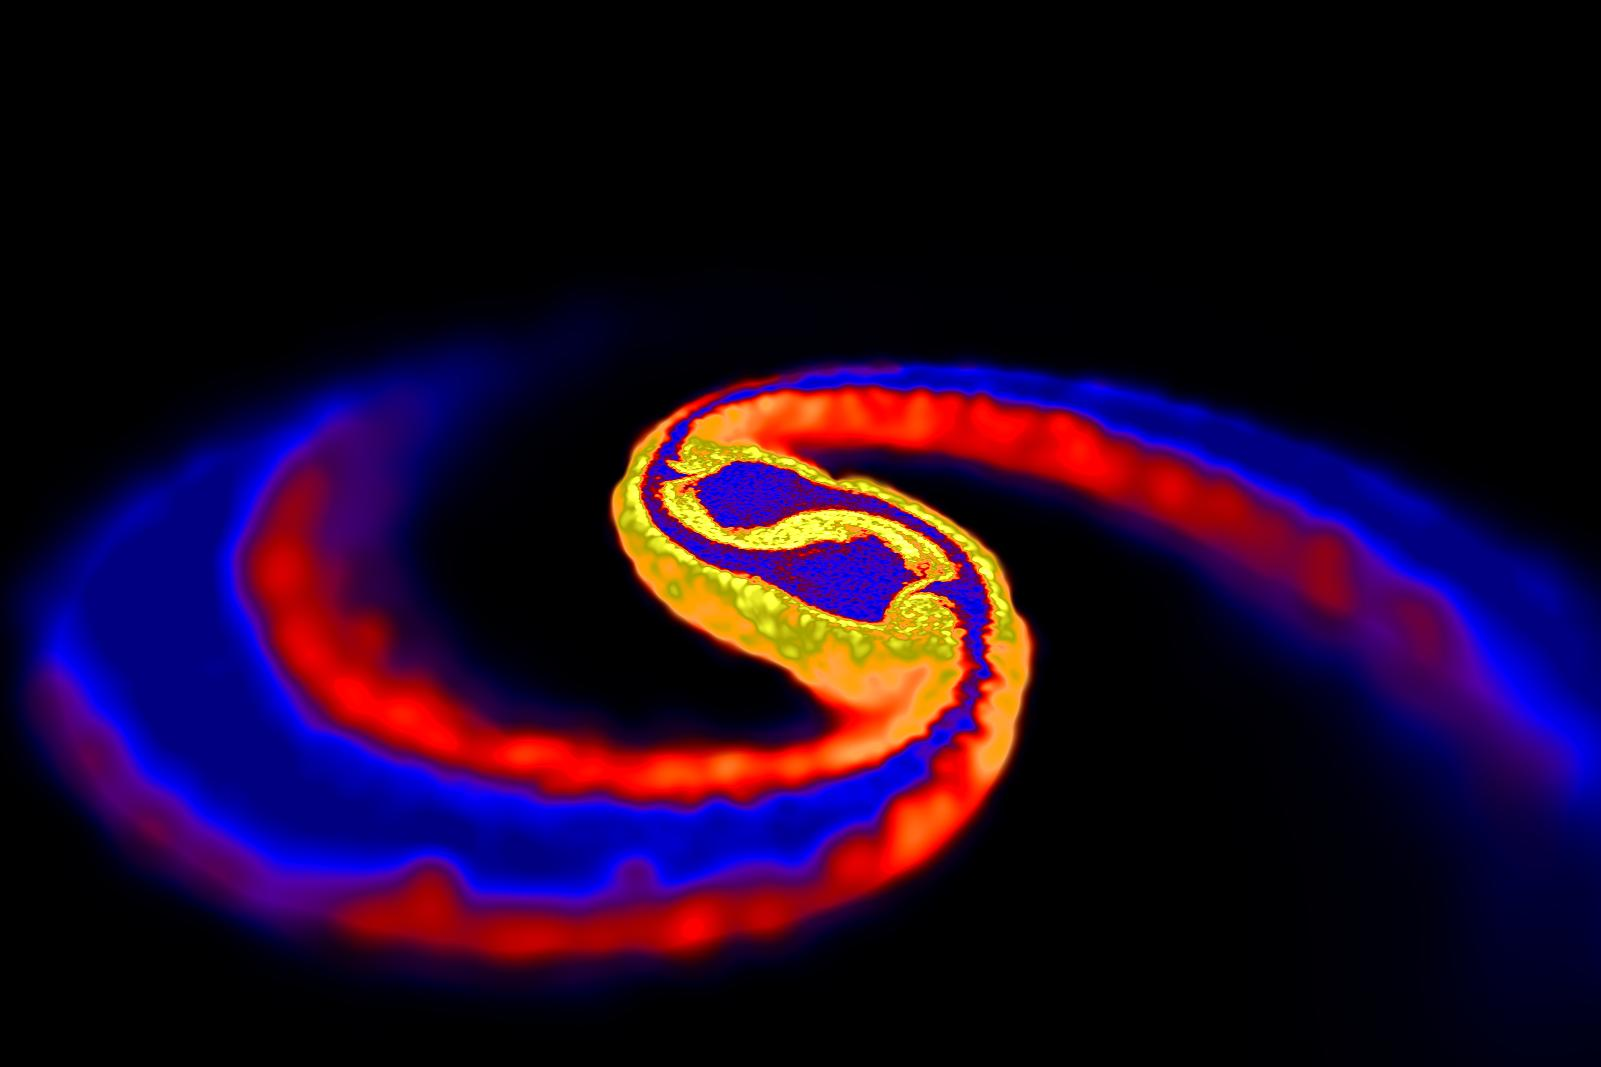
\includegraphics[width=\textwidth]{../images/price_rosswog_press_1}\\
\tiny Credit: Daniel Price (U/Exeter) and Stephan Rosswog (Int. U/Bremen)
\end{columns}
\end{frame}

\section{How do we model a neutron star?}
\begin{frame}
\frametitle{What features do we need to consider?}
\begin{columns}
\column{0.5\textwidth}
\begin{itemize}
\item{Exterior - Vacuum/Plasma}
\item{Atmosphere/Ocean - Fluid}
\item{Crust - Elastic Matter}
\item{Core - Fluid}
\end{itemize}
\column{0.6\textwidth}
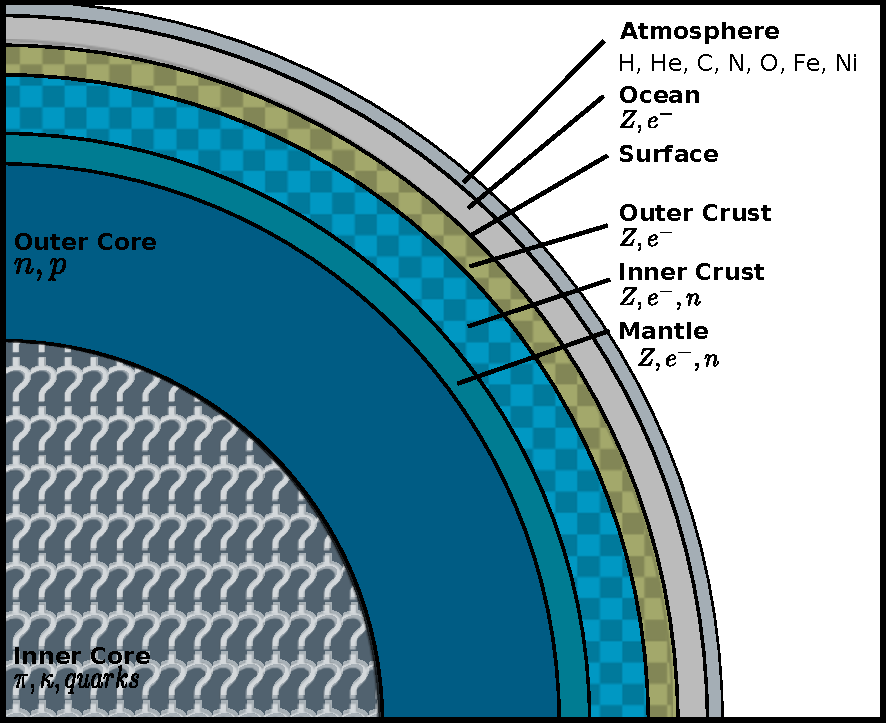
\includegraphics[width=\textwidth]{../images/neutron_star_structure}
\end{columns}
\end{frame}
\begin{frame}
\frametitle{How do we model a neutron star numerically?}
We want to solve the most realistic physical model possible using maximum resolution. Problem?
\begin{itemize}
\item{Important length-scales vary over 12 orders of magnitude if including viscous boundary layers.}
\item{Using adaptive mesh refinement cannot cover this range.}
\end{itemize}
Solution: \\
Relativistic multimodel approach developed by Millmore \& Hawke. \\
Approximate interfaces to be infinitely thin.
\end{frame}

\begin{frame}
\frametitle{The multimodel approach}
Simplify the most complex model by:
\begin{itemize}
\item{Taking appropriate limits in different regions of the domain.}
\begin{itemize}
\item{Force-free / Electro-vacuum / Multi-fluid MHD}
\item{Ideal MHD / Resistive MHD}
\item{Elasticity}
\end{itemize}
\item{Combining the different approximations with sharp interfaces.}
\item{Using evolution equations based on conservation laws.}
\begin{itemize}
\item{This allows us to accurately capture the locations of shock waves.}
\end{itemize}
\item{Moving the complicated physics to the interfaces.}
\begin{itemize}
\item{Boundary conditions are used to impose physics.}
\end{itemize}
\end{itemize}
This approach also allows a proper treatment of the surface. \\
Therefore, we no longer need a numerical atmosphere. 
\end{frame}

\begin{frame}
\frametitle{Conservation Laws}
The evolution equations are a system of non-linear partial differential equations in conservation law form,
\begin{equation}
\frac{\partial \mathbf{q}(x,t)}{\partial x}  + \frac{\partial \mathbf{F}(\mathbf{q}(x,t))}{\partial x} = 0,
\end{equation}
where $\mathbf{q}$ are the conserved variables and $\mathbf{F}$ are the fluxes.\\
The numerical update is then given by,
\begin{equation}
q^{n+1}_i = q^n_i + \frac{\Delta t}{\Delta x} \left(F^n_{i-1/2} - F^n_{i+1/2}\right),
\end{equation}
where $n$ is the time index and $i$ is the spatial index.
\end{frame}

\begin{frame}
\frametitle{Numerical Grid}
\begin{columns}
\column{0.45\textwidth}
\begin{itemize}
\item{We define a grid on which to evolve our models.}
\item{The red line indicates the true interface.}
\item{The white line indicates the numerical interface.}
\end{itemize}
\column{0.55\textwidth}
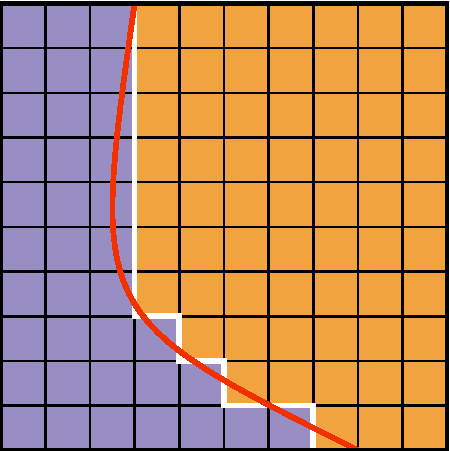
\includegraphics[width=\textwidth]{../images/multimodel_captured.pdf}
\end{columns}
\end{frame}

\begin{frame}
\frametitle{Moving Interface}
\begin{columns}
\column{0.45\textwidth}
\begin{itemize}
\item{The interface is advected with the physical velocity from the models.}
\item{The numerical interface tracks the physical interface.}
\item{Points can change model.}
\end{itemize}
\column{0.55\textwidth}
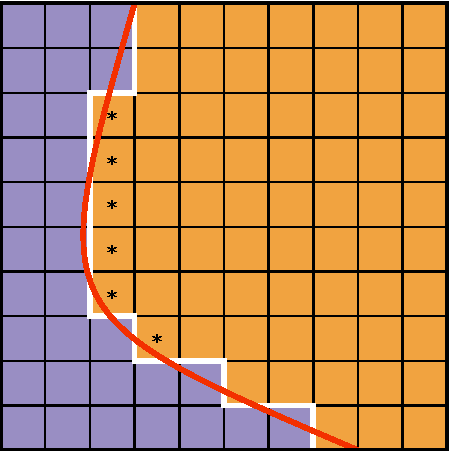
\includegraphics[width=\textwidth]{../images/multimodel_captured_2.pdf}
\end{columns}
\end{frame}

\begin{frame}
\frametitle{Ghost Zones}
\begin{columns}
\column{0.45\textwidth}
\begin{itemize}x
\item{Each model has a region of ghost zones.}
\item{As the update of each point is non-local, it is important to fill these cells correctly.}
\item{How do we impose the correct boundary conditions? By filling the ghost cells.}
\end{itemize}
\column{0.55\textwidth}
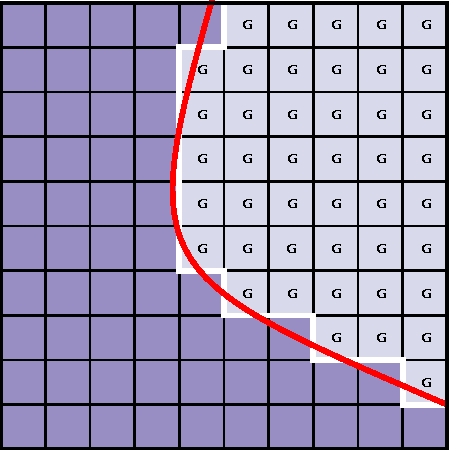
\includegraphics[width=\textwidth]{../images/multimodel_ghostcells.pdf}
\end{columns}
\end{frame}

\begin{frame}
\frametitle{Riemann Problem and Solution}
\begin{columns}
\column{0.5\textwidth}
\begin{itemize}
\item{Each normal cell is updated by following the Godunov approach.}
\item{Each cell boundary is a Riemann problem.}
\item{A Riemann problem occurs when there is a discontinuity.}
\item{We update each cell by calculating the flux through the boundaries.}
\end{itemize}
\column{0.6\textwidth}
\centering
Hydro Riemann Fan
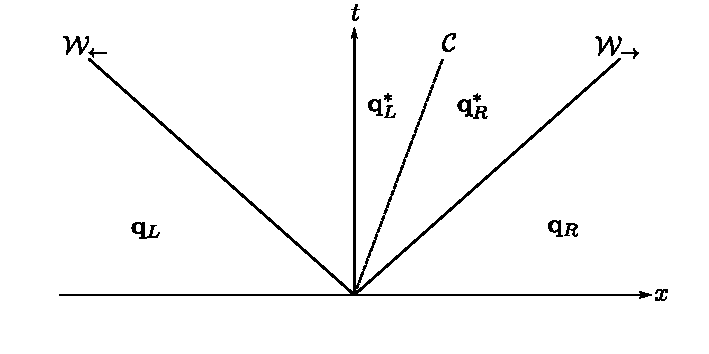
\includegraphics[width=\textwidth]{../images/euler_wave.pdf}
\end{columns}
\end{frame}

\begin{frame}
\frametitle{Riemann Problem and Solution}
\begin{columns}
\column{0.5\textwidth}
\begin{itemize}
\item{Each normal cell is updated by following the Godunov approach.}
\item{Each cell boundary is a Riemann problem.}
\item{A Riemann problem occurs when there is a discontinuity.}
\item{We update each cell by calculating the flux through the boundaries.}
\end{itemize}
\column{0.6\textwidth}
\centering
SRMHD Riemann Fan
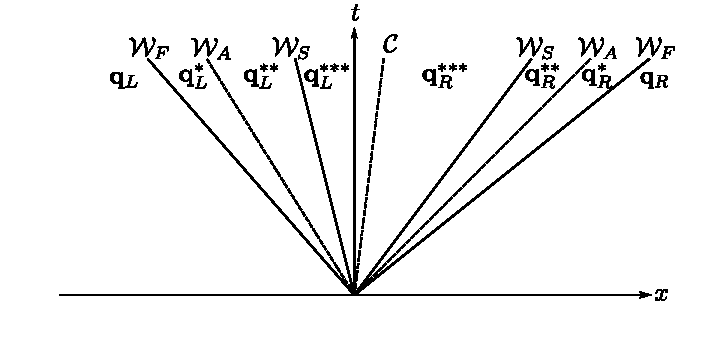
\includegraphics[width=\textwidth]{../images/srmhd_wave.pdf}
\end{columns}
\end{frame}

\section{Interfaces and Boundary Conditions}

\begin{frame}{Boundary Conditions: Ghost Fluid Method}
\begin{columns}
\column{6.5cm}
\centering
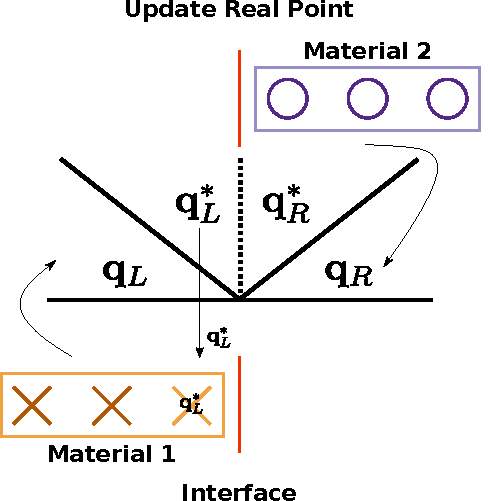
\includegraphics[width=6.5cm]{../images/multimodel_roe_real}
\column{4.5cm}
Follow the ghost fluid approach.
\begin{itemize}
\item{Define left and right states.}
\item{Calculate the star states using an appropriate method.}
\item{Fill the points neighbouring the interface.}
\item{Extrapolate into the ghost zones.}
\end{itemize}
\end{columns}
\end{frame}
\begin{frame}{Boundary Conditions: Ghost Fluid Method}
\begin{columns}
\column{6.5cm}
\centering
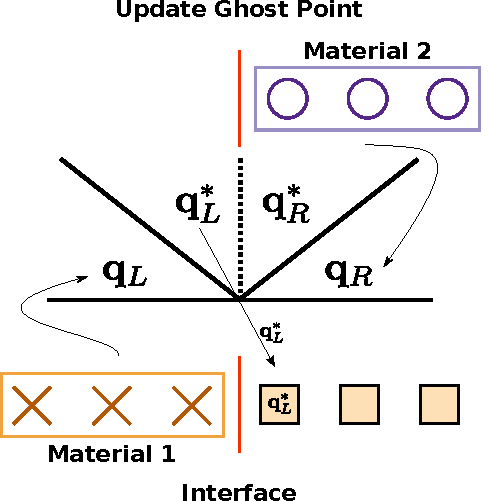
\includegraphics[width=6.5cm]{../images/multimodel_roe_ghost}
\column{4.5cm}
Follow the ghost fluid approach.
\begin{itemize}
\item{Define left and right states.}
\item{Calculate the star states using an appropriate method.}
\item{Fill the points neighbouring the interface.}
\item{Extrapolate into the ghost zones.}
\end{itemize}
\end{columns}
\end{frame}
\begin{frame}{Boundary Conditions: Ghost Fluid Method}
\begin{columns}
\column{6.5cm}
\centering
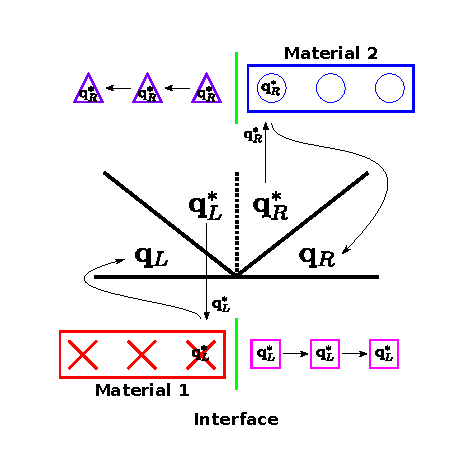
\includegraphics[width=6.5cm]{../images/multimodel_roe}
\column{4.5cm}
Follow the ghost fluid approach.
\begin{itemize}
\item{Define left and right states.}
\item{Calculate the star states using an appropriate method.}
\item{Fill the points neighbouring the interface.}
\item{Extrapolate into the ghost zones.}
\end{itemize}
\end{columns}
\end{frame}

\begin{frame}
\frametitle{How do we calculate the star states?}
Follow the Roe approximation method: linearise about an appropriate state $\mathbf{w}_X(\mathbf{q}_X)$ for the left and right states, where $X = L/R$,
\begin{equation}
\partial_t\mathbf{w}_X + \hat{A}_X\partial_{\mathnormal{x}}\mathbf{w}_X = 0.
\end{equation}
The star states are then given by the following equations,
\begin{align}
\mathbf{w}^*_L &= \mathbf{w}_L+\sum^{N_L}_{i=1}c^L_{i}\mathbf{r}^{(i)}_L,\\
\mathbf{w}^*_R &= \mathbf{w}_R-\sum^{N_R}_{j=1}c^R_{j}\mathbf{r}^{(j)}_R,
\end{align}
where $\mathbf{r}_X$ are the right eigenvectors of the matrix $\hat{A}_X$.
\end{frame}

\begin{frame}
\frametitle{How do we impose the interface boundary conditions?}
To calculate the coefficients $c^X$ we need  $N = N_L + N_R$ compatibility conditions at the interface, where $N_X$ is the number of waves between the initial and star state.\\
Through these compatibility conditions we impose the correct physical boundary conditions at the interface.\\
We assume that these compatibility conditions take the form:

\begin{equation}
\Delta w_j = w^{*R}_j-w^{*L}_j = 0, \quad j = 1,\dots, N.
\end{equation}
This gives a linear system which we can easily solve,
\begin{equation}
\mathbf{w}_R - \mathbf{w}_L = \sum^{N_R}_{j=1}c^R_{j}\mathbf{r}^{(j)}_R +  \sum^{N_L}_{i=1}c^L_{i}\mathbf{r}^{(i)}_L.
\end{equation}
\end{frame}

\section{Results}

\begin{frame}
\frametitle{Vorticity Propagation - Low Magnetic Field $\beta = 1000$}
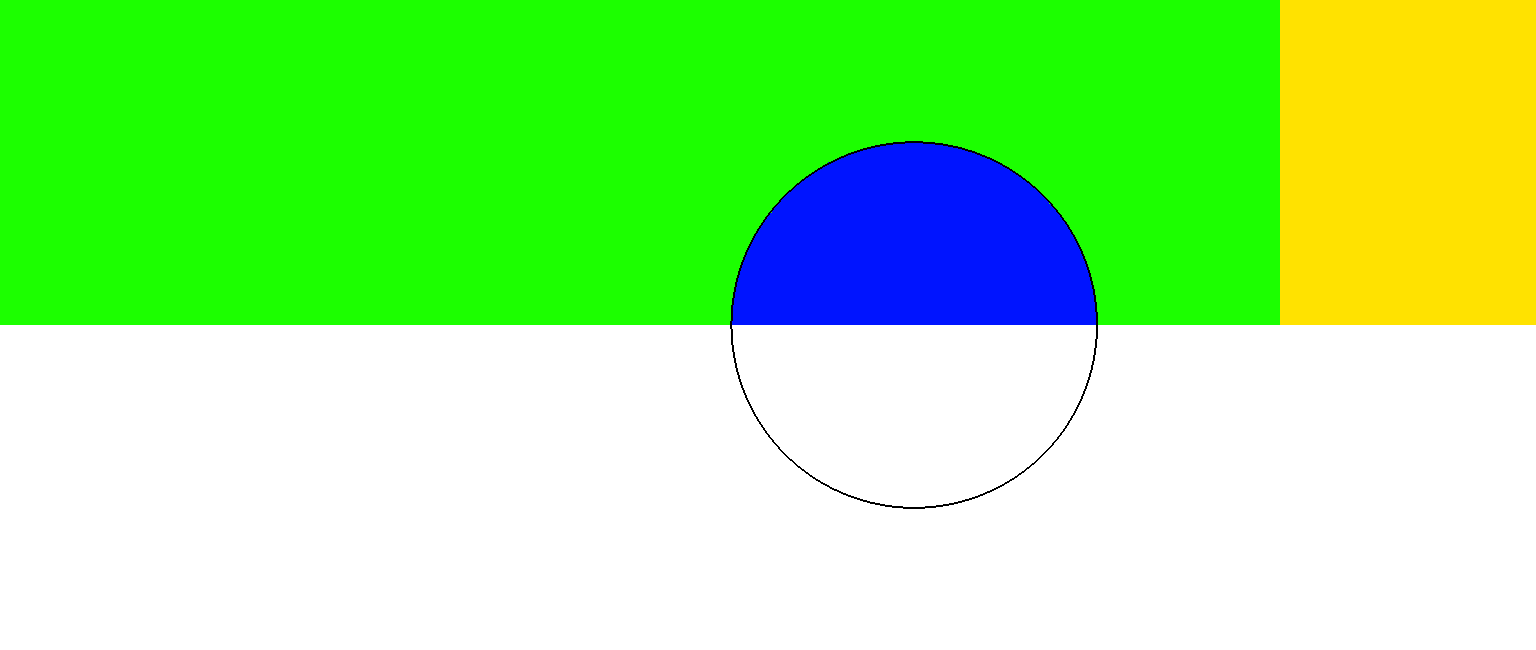
\includegraphics[width=\textwidth]{../images/SRMHDBubbleBeta1000_t0_crop.png}
\end{frame}

\begin{frame}
\frametitle{Vorticity Propagation - Low Magnetic Field $\beta = 1000$}

\includegraphics[width=\textwidth]{../images/SRMHDBubbleBeta1000_t31_crop.png}
\end{frame}

\begin{frame}
\frametitle{Vorticity Propagation - Low Magnetic Field $\beta = 1000$}
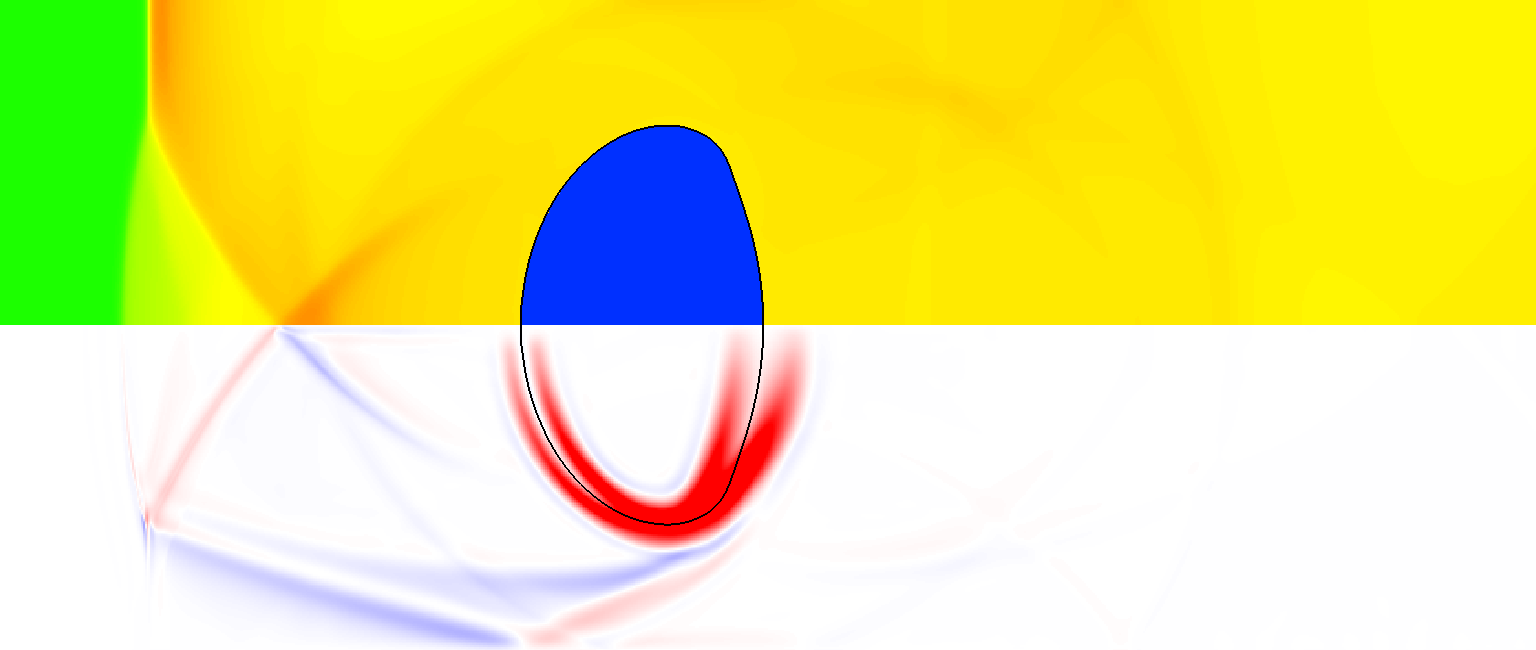
\includegraphics[width=\textwidth]{../images/SRMHDBubbleBeta1000_t59_crop.png}
\end{frame}

\begin{frame}
\frametitle{Vorticity Propagation - Low Magnetic Field $\beta = 1000$}
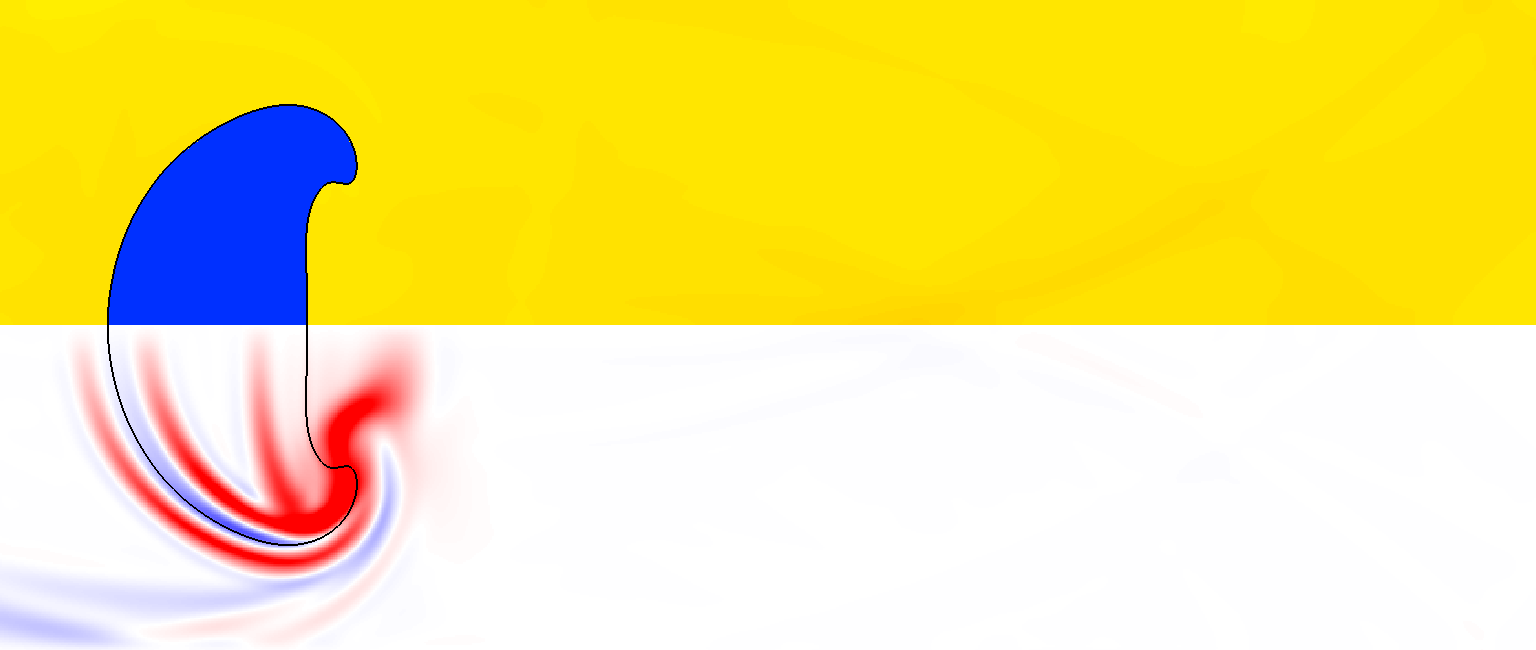
\includegraphics[width=\textwidth]{../images/SRMHDBubbleBeta1000_t125_crop.png}
\end{frame}

\begin{frame}
\frametitle{Vorticity Propagation - Low Magnetic Field $\beta = 1000$}
\begin{itemize}
\item{As with the hydrodynamical case, vorticity is produced at the interface.}
\item{In the presence of a magnetic field, the vorticity begins to detach.}
\item{Vorticity is propagated via the Alfv\'{e}n waves.}
\item{This occurs in the regime where the hydrodynamical pressure dominates the magnetic pressure.}
\end{itemize}
\end{frame}
\begin{frame}
\frametitle{Vorticity Propagation - Low Magnetic Field $\beta = 0.01$}
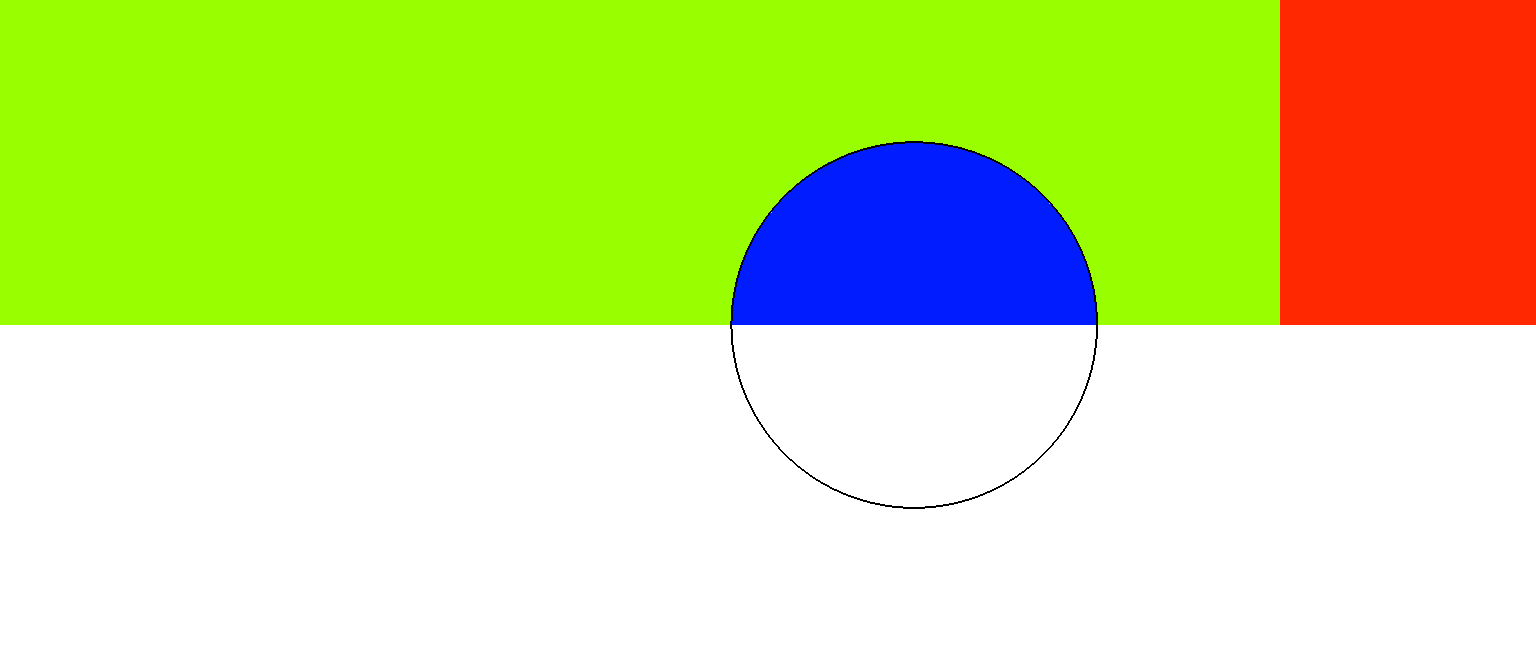
\includegraphics[width=\textwidth]{../images/SRMHDBubbleBeta001_t0_crop.png}
\end{frame}

\begin{frame}
\frametitle{Vorticity Propagation - Low Magnetic Field $\beta = 0.01$}
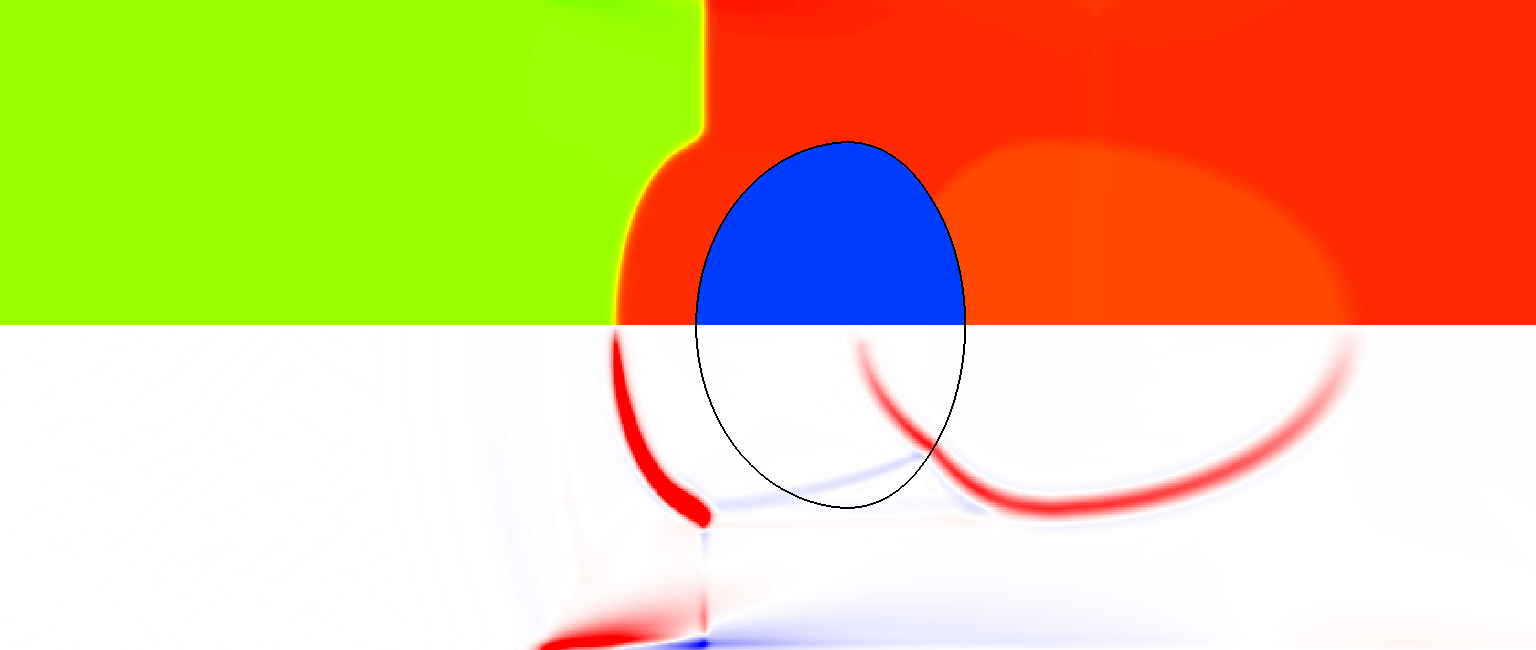
\includegraphics[width=\textwidth]{../images/SRMHDBubbleBeta001_t31_crop.png}
\end{frame}

\begin{frame}
\frametitle{Vorticity Propagation - Low Magnetic Field $\beta = 0.01$}
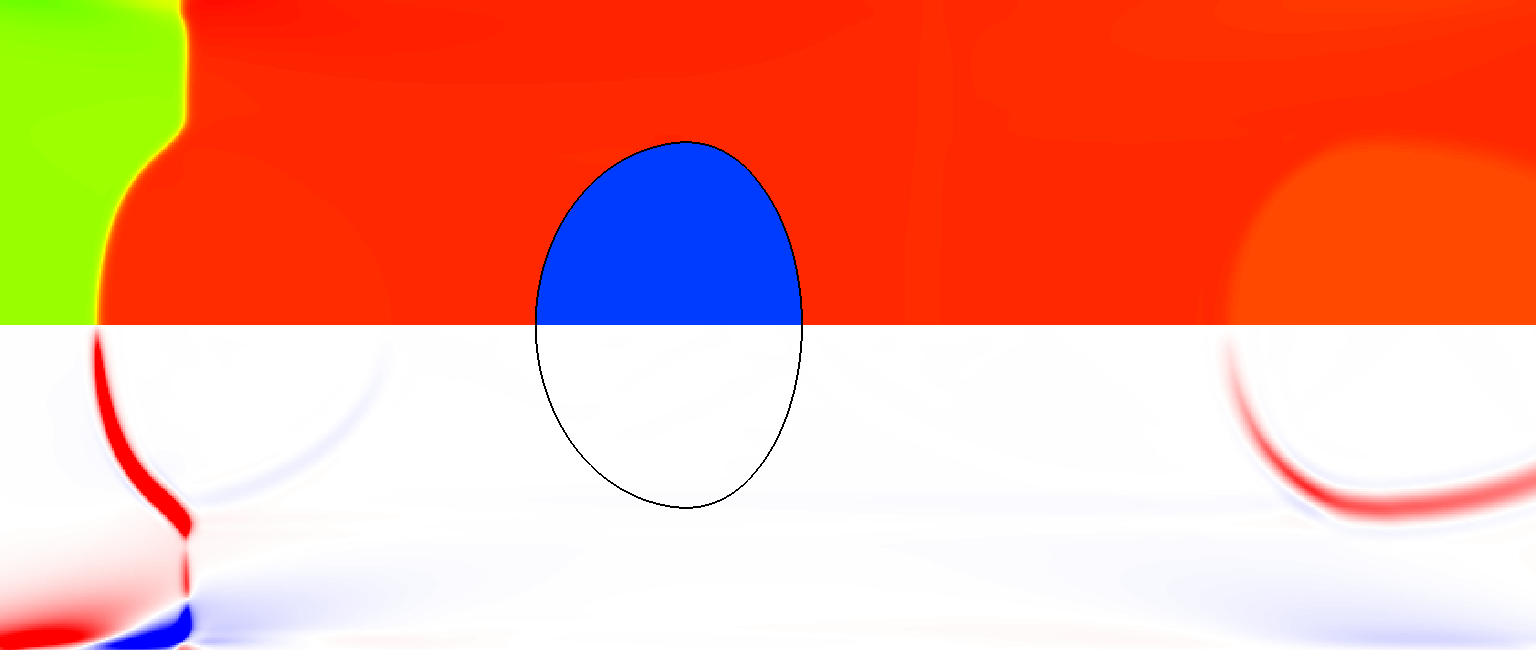
\includegraphics[width=\textwidth]{../images/SRMHDBubbleBeta001_t59_crop.png}
\end{frame}

\begin{frame}
\frametitle{Vorticity Propagation - Low Magnetic Field $\beta = 0.01$}
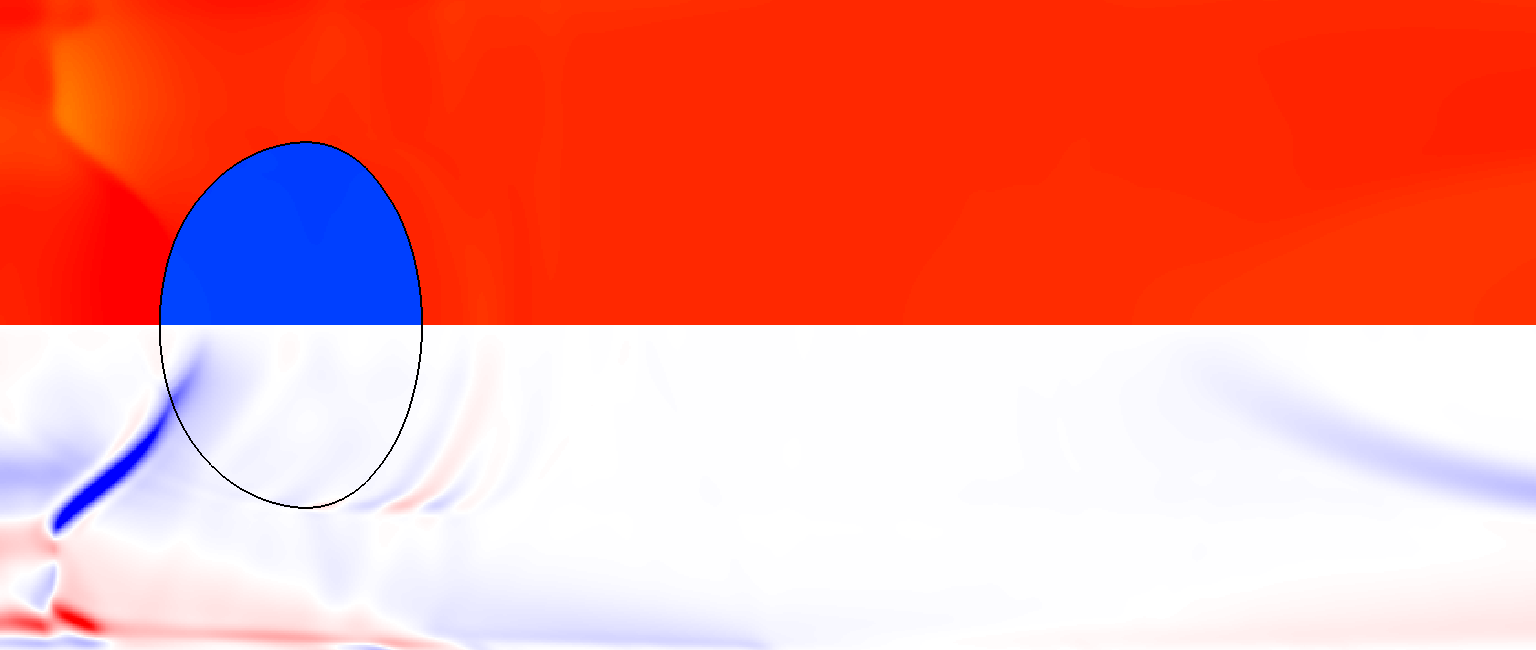
\includegraphics[width=\textwidth]{../images/SRMHDBubbleBeta001_t125_crop.png}
\end{frame}
\begin{frame}
\frametitle{Vorticity Propagation - Low Magnetic Field $\beta = 0.01$}
\begin{itemize}
\item{As with the low magnetic field case, vorticity is produced at the interface but is detached immediately.}
\item{It propagates away from the interface with the strongest waves.}
\item{This redistribution of vorticity and therefore angular momentum, when applied to a neutron star binary, will change the collapse time.}
\end{itemize}
\end{frame}

\begin{frame}
\frametitle{Toy Star: Vacuum - Hydro}
\begin{columns}
\column{0.55\textwidth}
\begin{itemize}
\item{Use Toy Star test of Price et al. to test vacuum boundary conditions with gravity.}
\item{We add gravity, as a source, into our evolution equations (purely Newtonian).}
\item{Evolving the density, we can see the star appears to be stable.}
\end{itemize}
\column{0.55\textwidth}
\centering
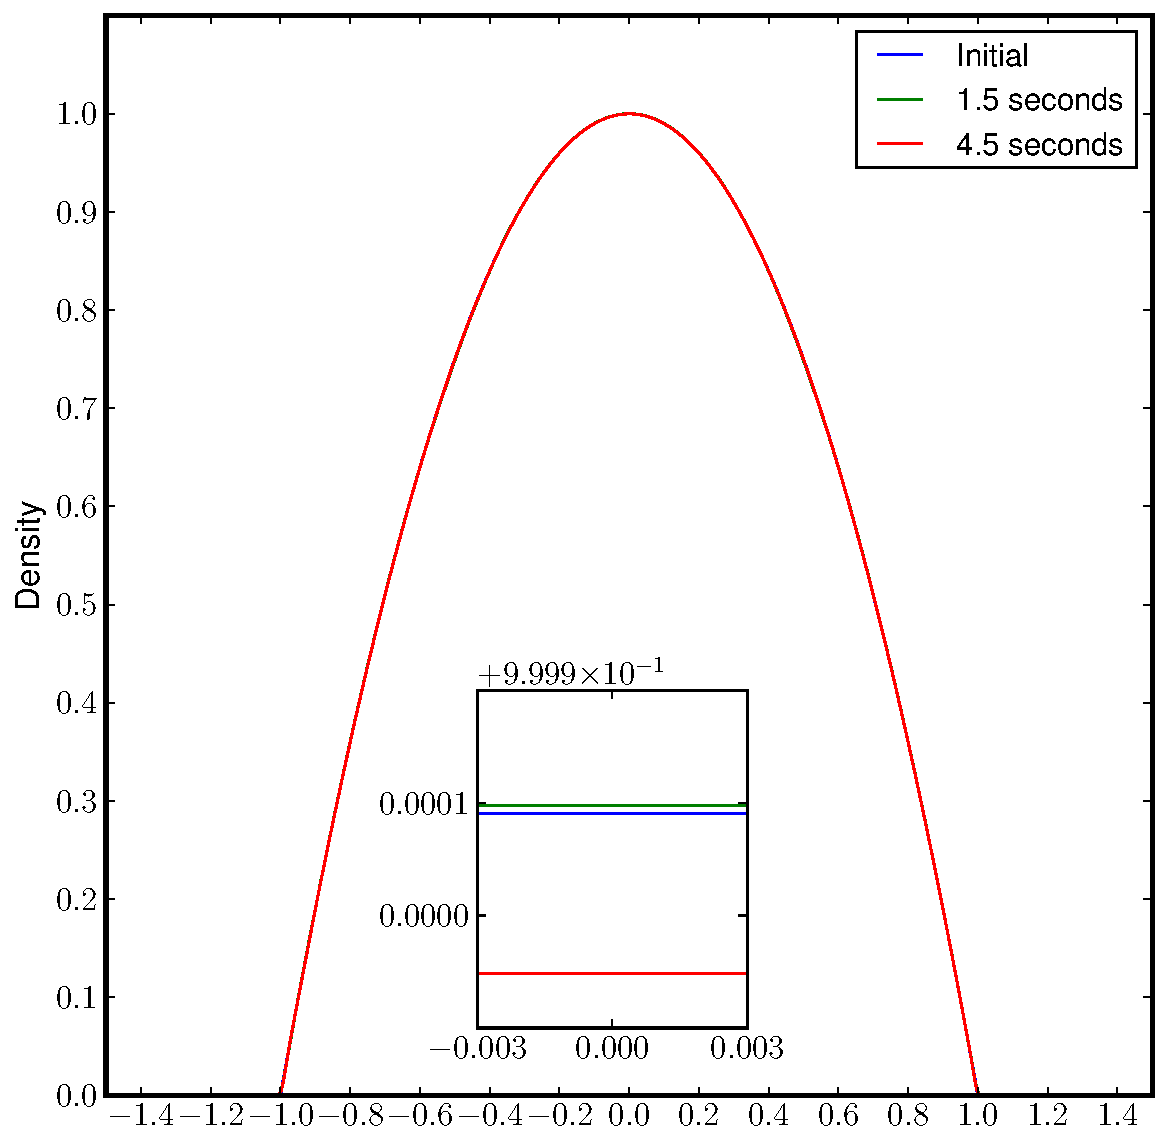
\includegraphics[width=\textwidth]{../images/toy_density}
\end{columns}
\end{frame}

%\begin{frame}
%\frametitle{Toy Star: Vacuum - Hydro}
%\begin{columns}
%\column{0.55\textwidth}
%\begin{itemize}
%\item{The velocity profile shows that the star is oscillating.}
%\item{The velocity increases at the edges due to the decrease in density.}
%\item{The velocity at the edges appears to be increasing!}
%\end{itemize}
%\column{0.55\textwidth}
%\centering
%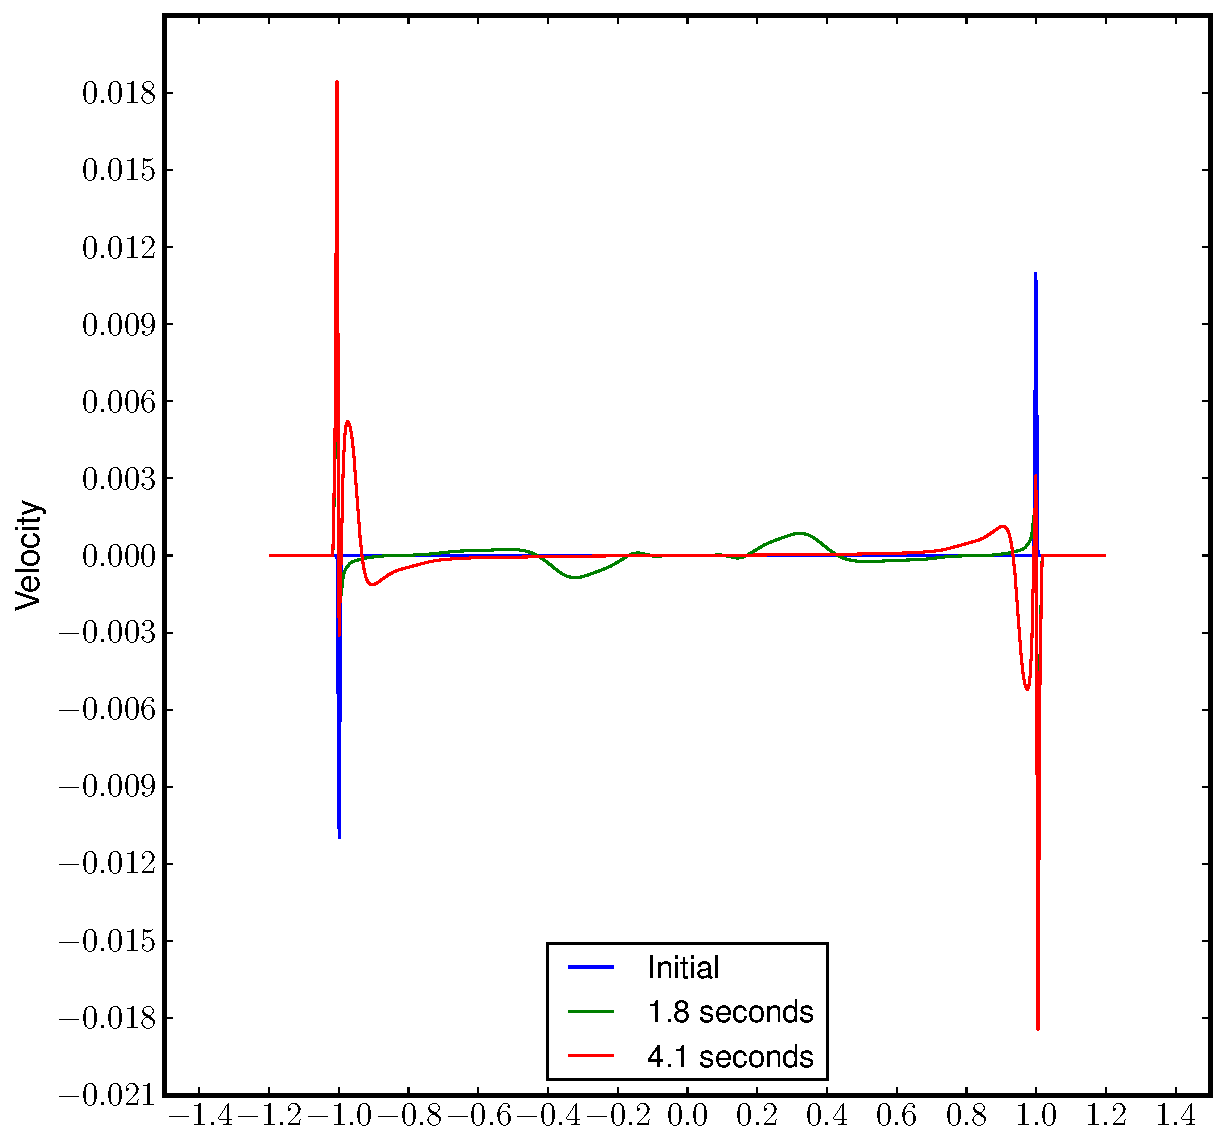
\includegraphics[width=\textwidth]{../images/toy_velocity}
%\end{columns}
%\end{frame}

\begin{frame}
\frametitle{Toy Star: Vacuum - Hydro}
\begin{columns}
\column{0.55\textwidth}
\begin{itemize}
\item{Over a longer time period, we can see the maximum velocity is decreasing.}
\item{The occurs even when the radius of the star increases.}
\item{We measured a characteristic time scale that is within $9\%$ of the expected value.}
\item{We believe this error is due to sampling and discretisation errors.}
\end{itemize}
\column{0.55\textwidth}
\centering
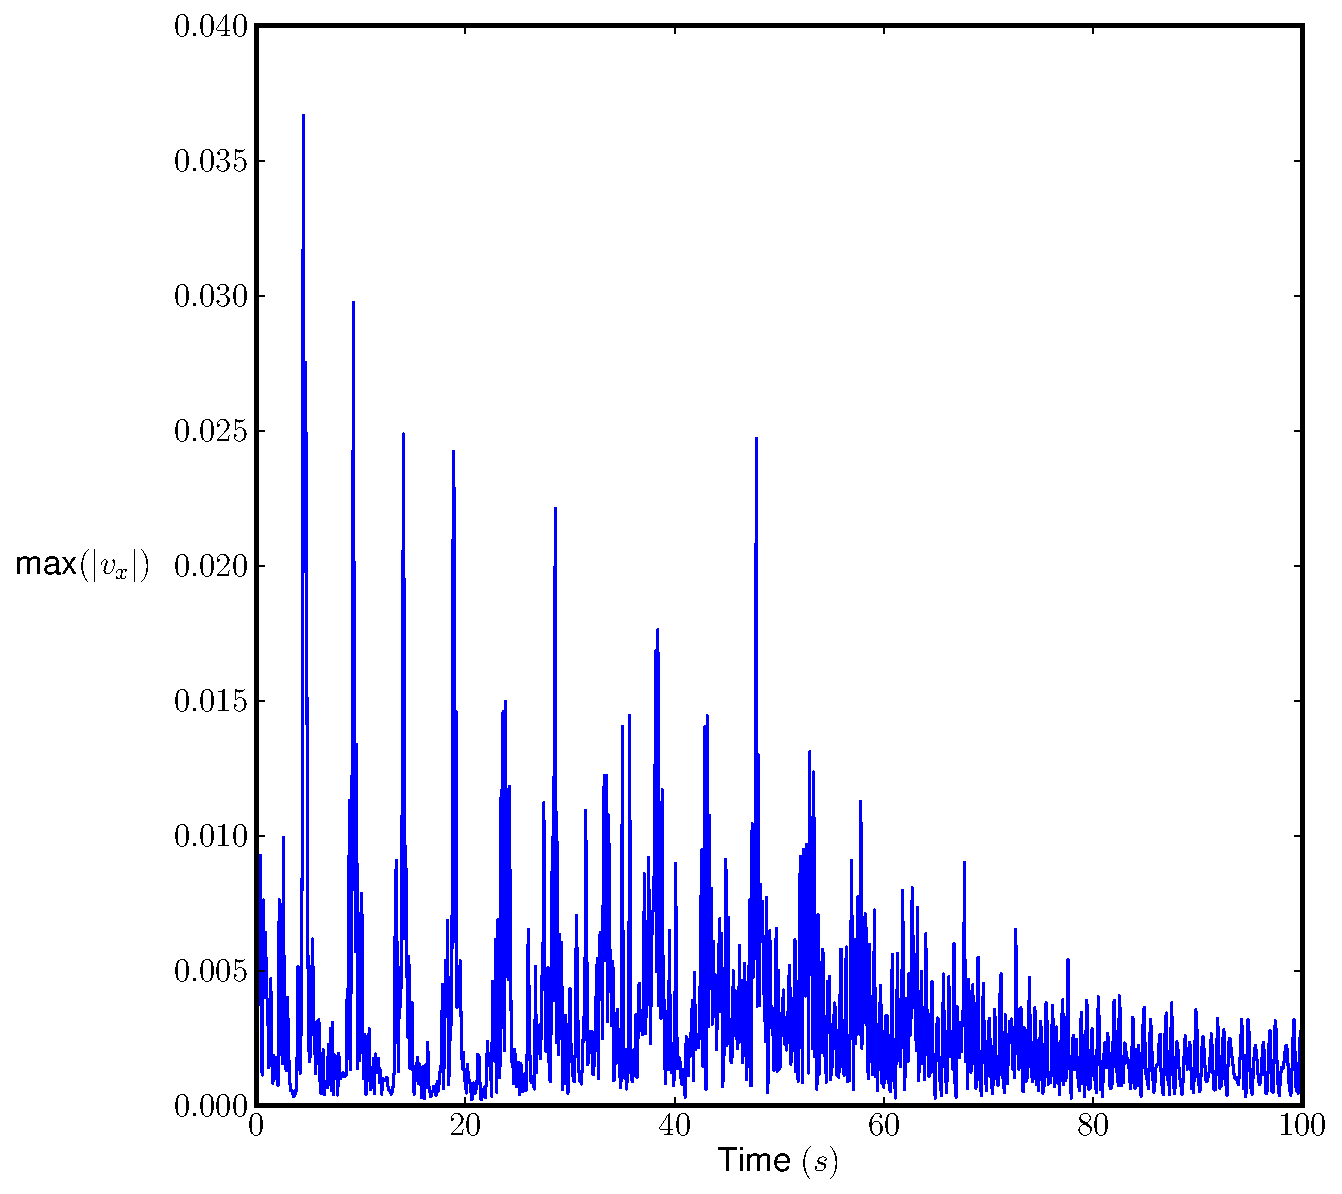
\includegraphics[width=\textwidth]{../images/toy_max_vx}
\end{columns}
\end{frame}

\section{Conclusion}
\begin{frame}
\frametitle{Conclusion}
\begin{itemize}
\item{We have developed a new approach for combining different systems of conservation laws.}
\item{We have applied this to relativistic Ideal MHD and shown that vorticity propagates away from interfaces via the Alfv\'{e}n waves.}
\item{These shock bubble tests have also been performed at Mach 40 and been shown to be robust.}
\item{We have also shown that this approach can be applied to vacuum interfaces in the presence of gravity.}
\end{itemize}
\end{frame}
\begin{frame}
\frametitle{Conclusion}
\centering
Thank you for listening.\\
Any Questions?
\end{frame}
\end{document}

